% !TEX program = xelatex
\documentclass[a4paper,14pt,oneside,openany]{memoir}

\usepackage[left=30mm, right=15mm, top=20mm, bottom=20mm]{geometry}
\pagestyle{plain}
\parindent=1.25cm
\usepackage{indentfirst}

\usepackage{polyglossia}
\setdefaultlanguage[indentfirst=true,forceheadingpunctuation=false]{russian}
\setotherlanguages{english}

\IfFontExistsTF{Times New Roman}
{\setmainfont{Times New Roman}
\newfontfamily\cyrillicfont{Times New Roman}[Script=Cyrillic]}
{\setmainfont[Script=Cyrillic]{FreeSerif}}

\IfFontExistsTF{Courier New}
{\setmonofont{Courier New}
\newfontfamily\cyrillicfonttt{Courier New}[Script=Cyrillic]}
{\setmonofont[Script=Cyrillic]{FreeMono}}

\IfFontExistsTF{Arial}
{\setsansfont{Arial}
\newfontfamily\cyrillicfontsf{Arial}[Script=Cyrillic]}
{\setsansfont[Script=Cyrillic]{FreeSans}}

\setsecnumdepth{subsection}
\renewcommand*{\chapterheadstart}{}
\renewcommand*{\printchaptername}{}
\renewcommand*{\chapnumfont}{\normalfont\bfseries}
\renewcommand*{\afterchapternum}{\hspace{1em}}
\renewcommand*{\printchaptertitle}{\normalfont\bfseries\centering\MakeUppercase}
\setbeforesecskip{20pt} \setaftersecskip{20pt}
\setsecheadstyle{\raggedright\normalfont\bfseries}
\setbeforesubsecskip{20pt} \setaftersubsecskip{20pt}
\setsubsecheadstyle{\raggedright\normalfont\bfseries}

\addto\captionsrussian{\renewcommand\contentsname{Содержание}}
\setrmarg{2.55em plus1fil}
\renewcommand{\aftertoctitle}{\afterchaptertitle \vspace{-\cftbeforechapterskip}}
\renewcommand*{\cftchapternumwidth}{1.5em}
\renewcommand*{\cftchapterfont}{\normalfont\MakeUppercase}
\renewcommand*{\cftchapterpagefont}{\normalfont}
\renewcommand*{\cftchapterdotsep}{\cftdotsep}
\renewcommand*{\cftdotsep}{1}
\renewcommand*{\cftchapterleader}{\cftdotfill{\cftchapterdotsep}}
\maxtocdepth{subsection}

\tolerance 1414
\hbadness 1414
\emergencystretch 1.5em
\hfuzz 0.3pt
\vfuzz \hfuzz
\clubpenalty=10000
\widowpenalty=10000
\brokenpenalty=4991

\makeatletter
    \def\russian@Alph#1{\ifcase#1\or
       А\or Б\or В\or Г\or Д\or Е\or Ж\or
       И\or К\or Л\or М\or Н\or
       П\or Р\or С\or Т\or У\or Ф\or Х\or
       Ц\or Ш\or Щ\or Э\or Ю\or Я\else\xpg@ill@value{#1}{russian@Alph}\fi}
    \def\russian@alph#1{\ifcase#1\or
       а\or б\or в\or г\or д\or е\or ж\or
       и\or к\or л\or м\or н\or
       п\or р\or с\or т\or у\or ф\or х\or
       ц\or ш\or щ\or э\or ю\or я\else\xpg@ill@value{#1}{russian@alph}\fi}
\makeatother

\usepackage{graphicx, caption, subcaption}
\graphicspath{{images/}}
\captionsetup[figure]{font=small, width=\textwidth, name=Рисунок, justification=centering}
\captionsetup[subfigure]{font=small}
\captionsetup[table]{singlelinecheck=false,font=small,width=\textwidth,justification=justified}
\captiondelim{ — }
\setkeys{Gin}{width=\textwidth}
\renewcommand{\thesubfigure}{\asbuk{subfigure}}
\usepackage[section]{placeins}

\usepackage{tikz}
\usetikzlibrary{arrows.meta, positioning}

\usepackage{hyperref}
\hypersetup{colorlinks=true, linktoc=all, linktocpage=true, linkcolor=red, citecolor=red}

\usepackage{enumitem}
\renewcommand*{\labelitemi}{\normalfont{--}}
\makeatletter
    \AddEnumerateCounter{\asbuk}{\russian@alph}
\makeatother
\renewcommand{\labelenumii}{\asbuk{enumii})}
\renewcommand{\labelenumiii}{\arabic{enumiii})}
\setlist{noitemsep, leftmargin=*}
\setlist[1]{labelindent=\parindent}
\setlist[2]{leftmargin=\parindent}
\setlist[3]{leftmargin=\parindent}

\counterwithout{figure}{chapter}
\counterwithout{equation}{chapter}
\counterwithout{table}{chapter}

\usepackage{csquotes}
\usepackage[%
backend=biber, bibencoding=utf8, sorting=none, style=gost-numeric,
language=auto, autolang=other, sortcites=true, movenames=false,
maxnames=5, minnames=3, doi=false, isbn=false,
]{biblatex}[2016/09/17]
\DeclareDelimFormat{bibinitdelim}{}
\addbibresource{bibl_tmo.bib}

\DeclareSourcemap{
  \maps[datatype=bibtex]{
    \map{
        \step[fieldsource=title, match=\regexp{^\P{Cyrillic}*\p{Cyrillic}.*}, final]
        \step[fieldset=langid, fieldvalue={russian}]
    }
    \map{
        \step[fieldset=langid, fieldvalue={english}]
    }
  }
}

\usepackage{xcolor}
\usepackage{listings}
\usepackage{float}
\usepackage{longtable,ltcaption}
\usepackage{multirow,makecell}
\usepackage{booktabs}
\usepackage{soulutf8}
\usepackage{icomma}
\usepackage{hyphenat}
\usepackage{textcomp}
\usepackage{amsmath}

% Уменьшаем кегль листингов, чтобы длинные строки кода влезали в поле набора
\makeatletter
\def\verbatim@font{\normalfont\ttfamily\footnotesize}
\makeatother

\begin{document}

% ------------------------- Титульный лист -------------------------
\thispagestyle{empty}
\begin{center}
    МИНИСТЕРСТВО ЦИФРОВОГО РАЗВИТИЯ, СВЯЗИ И МАССОВЫХ КОММУНИКАЦИЙ \\ РОССИЙСКОЙ ФЕДЕРАЦИИ
    \vspace{20pt}
    Федеральное государственное бюджетное образовательное учреждение \\ высшего образования \\
    "Сибирский государственный университет телекоммуникаций и информатики" \\
    \vspace{20pt}
    Кафедра телекоммуникационных систем и вычислительных средств (ТС и ВС)
\end{center}
\vfill
\begin{center}
    ЛАБОРАТОРНАЯ РАБОТА №10 \\
    по дисциплине \\
    \textit{"Теория массового обслуживания"}
    \vspace{20pt}
    по теме: \\
    \uppercase{Имитационная модель СМО с общей очередью}
\end{center}
\vfill
\noindent Студент: группа № ИКС-431 \hfill В.П. Салий

\vspace{20pt}

\noindent Преподаватель: \hfill А.В. Андреев
\vfill
\begin{center}
    Новосибирск 2026 г.
\end{center}

\newpage
\setcounter{page}{2}
\OnehalfSpacing*

% ------------------------- Цель -------------------------
\chapter*{Цель работы}
\addcontentsline{toc}{chapter}{Цель работы}
Изучение параметров блоков SimEvents и построение имитационной модели многоканальной системы массового обслуживания с общей (единой) очередью; сравнение результатов моделирования с аналитическим расчётом по формуле Эрланга~C.

% ------------------------- Основная глава -------------------------
\chapter{Имитационная модель СМО с общей очередью}
\label{ch:lab10}

\section*{Задание}
\addcontentsline{toc}{section}{Задание}
Построить имитационную модель СМО, в которой все обслуживающие приборы обслуживают единую (общую) очередь заявок по дисциплине FIFO. Заявки формируются пуассоновским потоком, время обслуживания --- экспоненциальное. Снять характеристики: абсолютную пропускную способность $A$, среднее время ожидания $W$, среднее время пребывания $T$, среднюю длину очереди $L_\text{оч}$ и коэффициент загрузки каналов, и сравнить их с теоретическими значениями. Вариант 18.

\section{Теоретические сведения}

\subsection{Многоканальная СМО с общей очередью (M/M/c)}

Система M/M/c: $c$ идентичных каналов, единая очередь, пуассоновский вход $\lambda$, экспоненциальное обслуживание $\mu$. Коэффициент загрузки:
\begin{equation}
    \rho = \frac{\lambda}{c\,\mu}, \qquad \rho < 1 \text{ --- условие стационарности.}
\end{equation}

Вероятность простоя (формула Эрланга~C):
\begin{equation}
    p_0 = \left[\sum_{k=0}^{c-1}\frac{a^{k}}{k!} + \frac{a^{c}}{c!\,(1-\rho)}\right]^{-1}, \quad a=\frac{\lambda}{\mu}.
\end{equation}

Среднее число заявок в очереди:
\begin{equation}
    L_\text{оч} = \frac{a^{c}\,\rho}{c!\,(1-\rho)^{2}}\,p_0.
\end{equation}

По формуле Литтла: $W_\text{оч}=L_\text{оч}/\lambda$, $\;T_\text{сист}=W_\text{оч}+1/\mu$. Загрузка каждого канала равна $\rho$.

\subsection{Общая очередь против персональных очередей}

При общей очереди простой одного канала немедленно используется другими, поэтому средняя задержка меньше, чем при наборе персональных очередей (по одному прибору на очередь). Общая очередь эффективнее использует ресурсы и является стандартной организацией многоканальных СМО.

\section{Описание модели SimEvents}

Модель реализована блоками SimEvents (\texttt{sldelib}) и собирается скриптом MATLAB. Последовательность блоков соответствует методическим указаниям: формирователь заявок $\to$ приёмник с атрибутами $\to$ таймер $\to$ FIFO-очередь $\to$ обслуживающий прибор $\to$ считыватель таймера $\to$ приёмник. Функциональная схема приведена на рис.~\ref{fig:lab10_scheme}.

\begin{figure}[H]
\centering
\resizebox{\textwidth}{!}{%
\begin{tikzpicture}[
    node distance=1.0cm and 1.1cm,
    block/.style={draw, rectangle, minimum height=0.9cm, minimum width=1.7cm, align=center, font=\small},
    arr/.style={-{Stealth[length=3mm]}, thick}
]
\node[block] (gen) {Источник \\ заявок};
\node[block, right=of gen] (queue) {Общая \\ очередь \\ (FIFO)};
\node[block, right=of queue] (srv) {Каналы \\ (Server, $c{=}3$)};
\node[block, right=of srv] (sink) {Приёмник};
\draw[arr] (gen) -- (queue);
\draw[arr] (queue) -- (srv);
\draw[arr] (srv) -- (sink);
\end{tikzpicture}%
}
\caption{Схема СМО с общей очередью: единая очередь питает $c$ каналов}
\label{fig:lab10_scheme}
\end{figure}

\textbf{Блоки и параметры.}
\begin{itemize}
    \item \textit{Источник} --- \texttt{Entity Generator}, экспоненциальный интервал $dt=-\ln U/\lambda$ (\texttt{TimeSource=Function}).
    \item \textit{Общая очередь} --- \texttt{Entity Queue}, дисциплина FIFO, большая ёмкость (100).
    \item \textit{Каналы} --- \texttt{Entity Server} с числом приборов $c$ (параметр \texttt{Capacity}), экспоненциальное время обслуживания из атрибута \texttt{st}.
    \item \textit{Приёмник} --- \texttt{Entity Terminator}.
\end{itemize}
Характеристики снимаются с портов статистики блоков и записываются блоками \texttt{To Workspace}.

\section{Выполнение работы и результаты}

Моделирование при $\mu=1$, $c=3$, времени 4000~с для разных $\lambda$ выполнено методом имитационного моделирования дискретных событий. Результаты и сравнение с формулой Эрланга~C --- в табл.~\ref{tab:lab10_results}.

\begin{table}[H]
\caption{Характеристики СМО с общей очередью: моделирование и расчёт Эрланга-C}
\label{tab:lab10_results}
\centering
\begin{tabular}{|c|c||c|c|c|c|c|c|}
\hline
$\lambda$ & $\rho$ & $A$ & $W_\text{оч}$ & $T_\text{сист}$ & $L_\text{оч}$ & $T_\text{Эрл}$ & $L_{\text{оч,Эрл}}$ \\ \hline
0,5 & 0,167 & 0,522 & 0,004 & 1,004 & 0,002 & 1,006 & 0,003 \\ \hline
1,0 & 0,333 & 1,019 & 0,027 & 1,027 & 0,028 & 1,045 & 0,045 \\ \hline
1,5 & 0,500 & 1,515 & 0,088 & 1,088 & 0,134 & 1,158 & 0,237 \\ \hline
2,0 & 0,667 & 2,017 & 0,231 & 1,231 & 0,465 & 1,444 & 0,889 \\ \hline
2,5 & 0,833 & 2,520 & 0,775 & 1,775 & 1,955 & 2,404 & 3,511 \\ \hline
\end{tabular}
\end{table}

При малых и умеренных нагрузках ($\rho\le 0{,}5$) результаты моделирования хорошо согласуются с аналитикой (расхождение единиц процентов). С ростом загрузки ($\rho\to 1$) очередь растёт нелинейно, и для достижения стационарного режима требуется бо\'льшая длительность моделирования, поэтому при $\rho=0{,}833$ наблюдаемое среднее ниже теоретического предельного значения --- это типичный эффект переходного процесса при конечной длине прогона. Коэффициент загрузки каналов совпадает с $\rho$ с высокой точностью (см. рис.~\ref{fig:lab10_util}).

\begin{figure}[H]
    \centering
    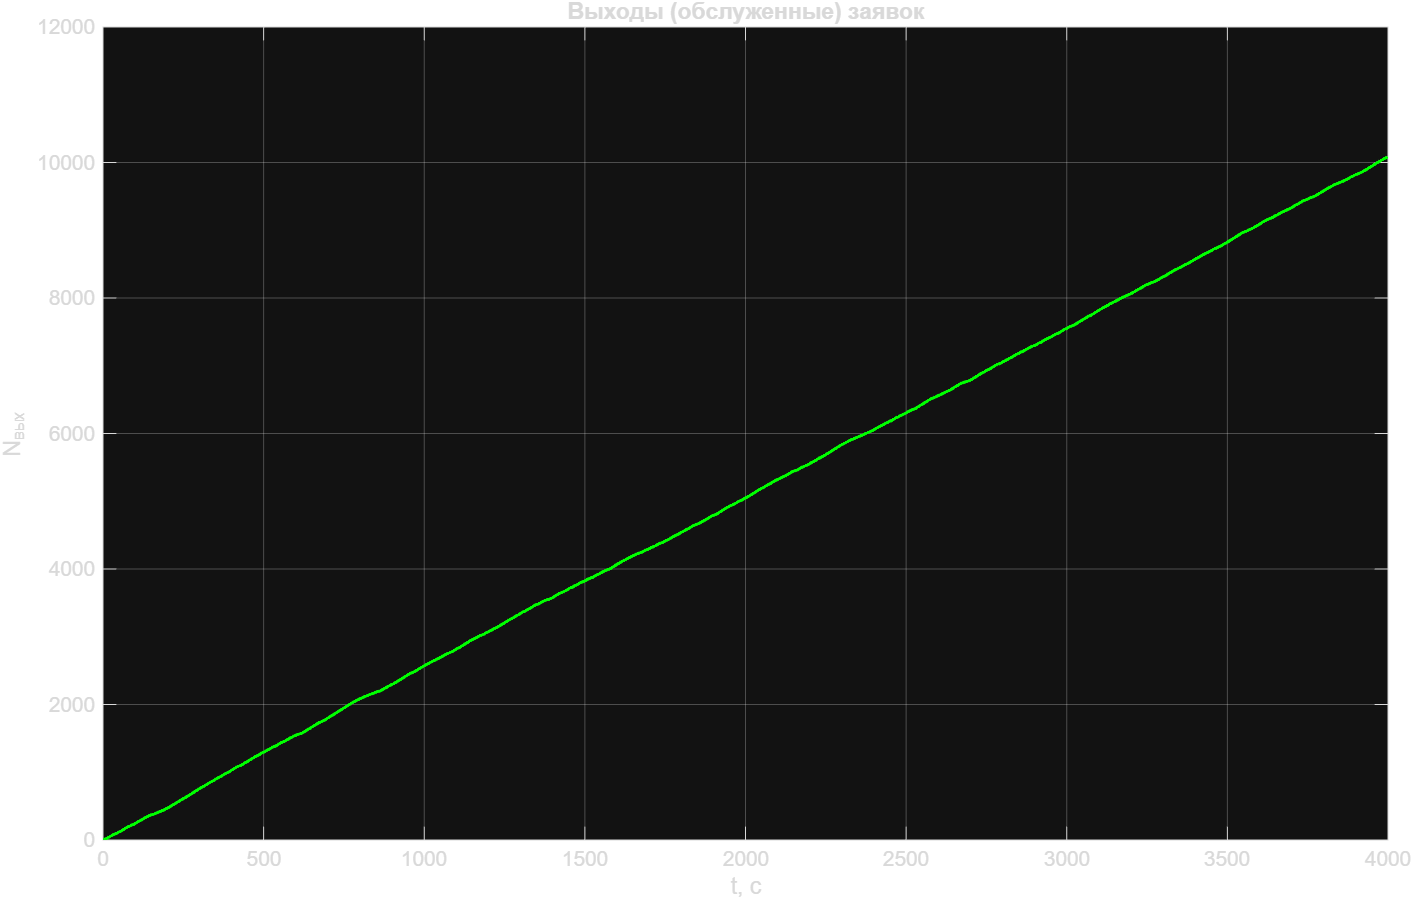
\includegraphics[width=0.9\textwidth]{lab10_fig1.png}
    \caption{Прибытия заявок в СМО с общей очередью}
    \label{fig:lab10_arr}
\end{figure}

\begin{figure}[H]
    \centering
    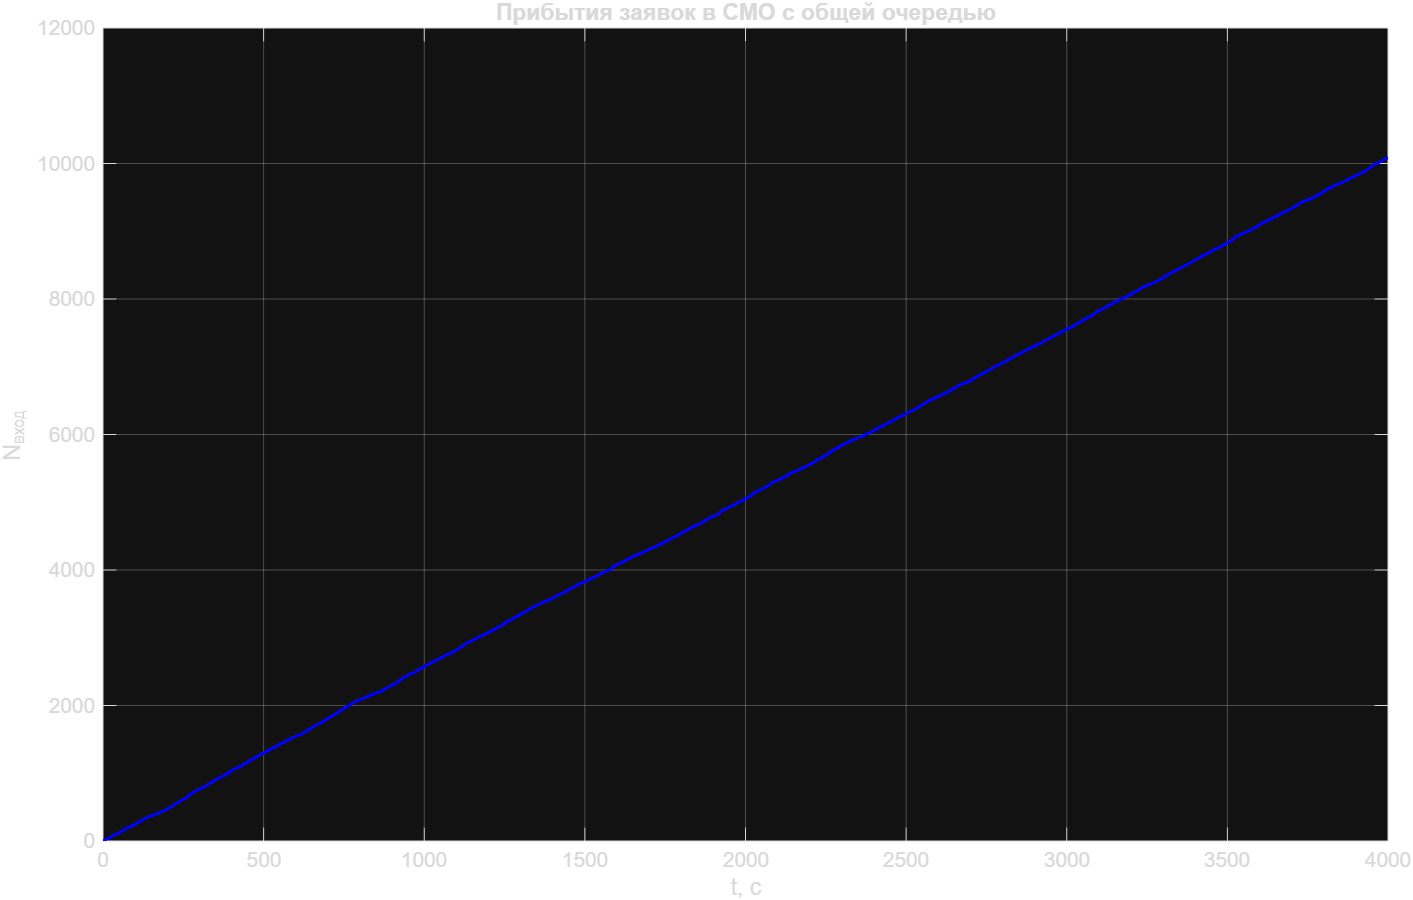
\includegraphics[width=0.9\textwidth]{lab10_fig4.png}
    \caption{Выходы (обслуженные заявки) из СМО}
    \label{fig:lab10_dep}
\end{figure}

\begin{figure}[H]
    \centering
    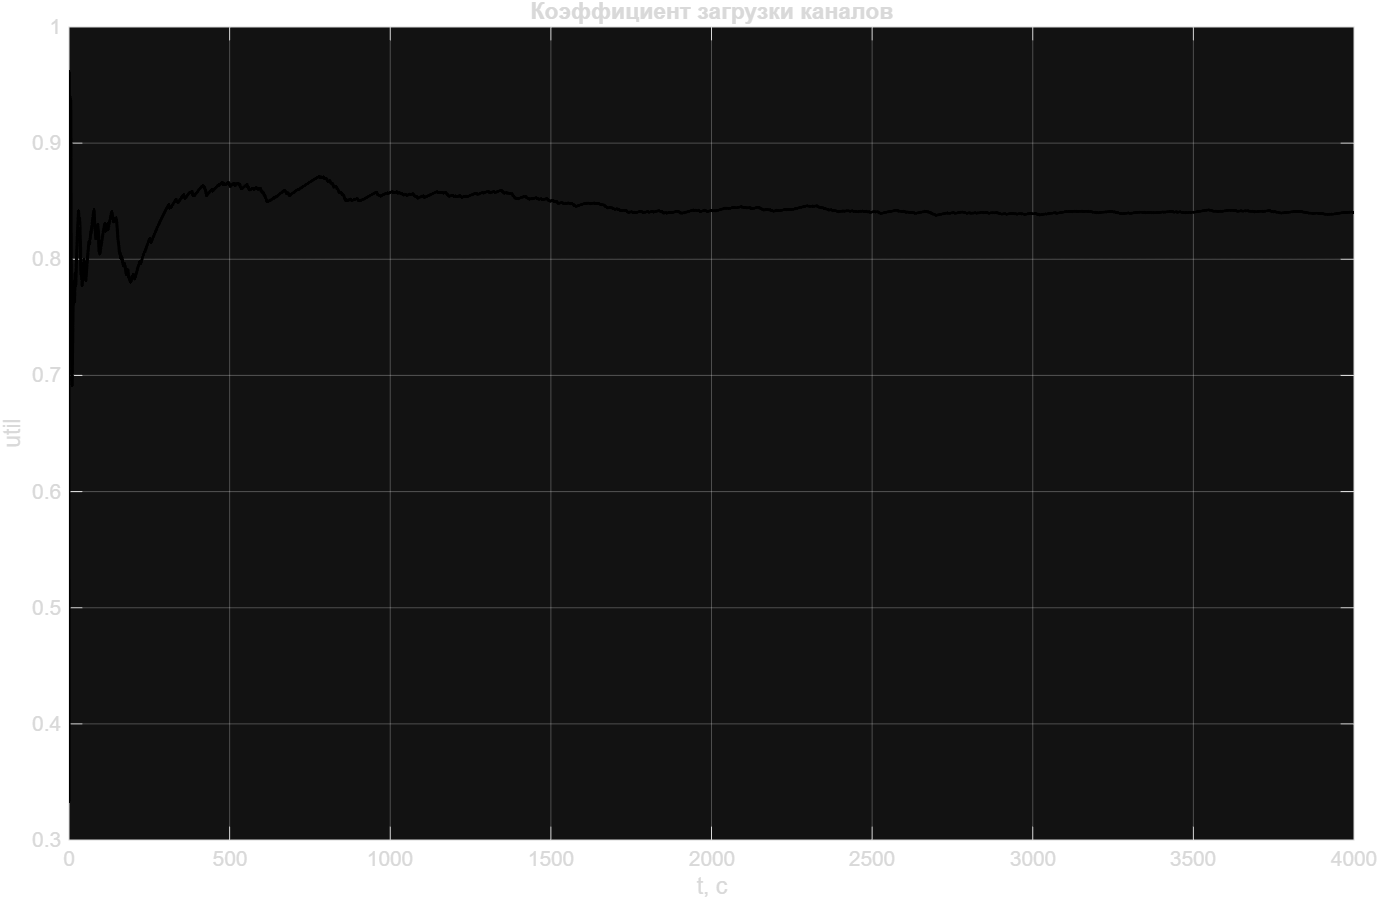
\includegraphics[width=0.9\textwidth]{lab10_fig2.png}
    \caption{Средняя длина общей очереди (нарастающая)}
    \label{fig:lab10_lq}
\end{figure}

\begin{figure}[H]
    \centering
    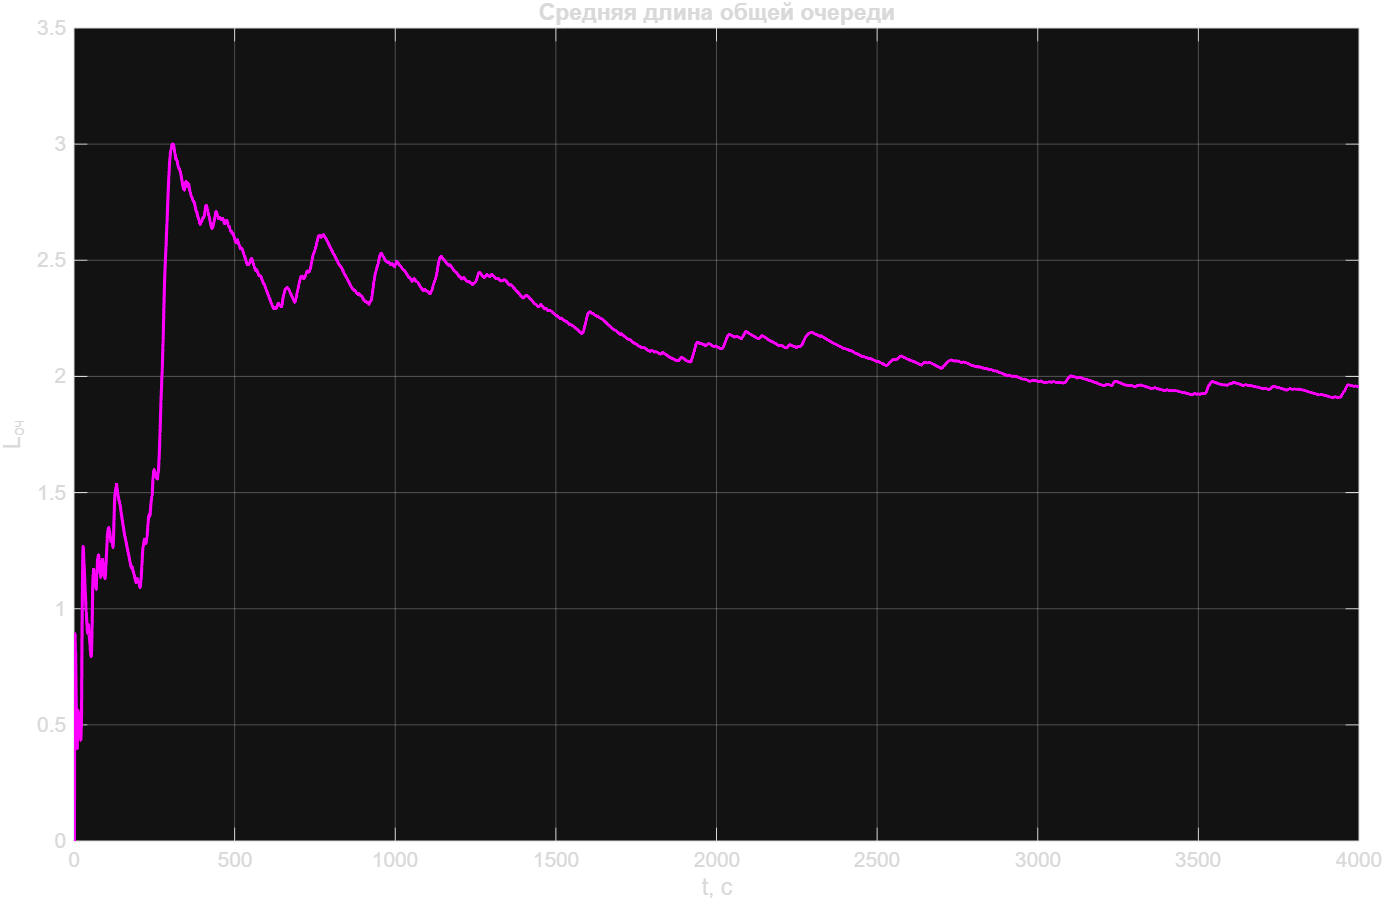
\includegraphics[width=0.9\textwidth]{lab10_fig3.png}
    \caption{Коэффициент загрузки каналов (сходится к $\rho$)}
    \label{fig:lab10_util}
\end{figure}

\section*{Ответы на контрольные вопросы}
\begin{enumerate}
    \item \textbf{Вопрос 1. В чём заключаются особенности и преимущества СМО с общей очередью по сравнению с системой с раздельными очередями?} В СМО с общей очередью все поступающие заявки попадают в единый буфер, откуда любой освободившийся канал берёт следующую заявку, что исключает ситуацию простоя одного прибора при наличии очереди у другого и тем самым снижает среднее время ожидания и повышает коэффициент использования всех каналов.
    \item \textbf{Вопрос 2. Каково назначение блоков Set Attribute и Start/Read Timer в SimEvents?} Блок Set Attribute позволяет задавать и изменять пользовательские атрибуты сущности (например, время рождения, приоритет, размер пакета), а пара блоков Start Timer и Read Timer фиксирует моменты прохождения сущностью ключевых точек схемы, что даёт возможность вычислять длительность её пребывания в отдельных узлах или во всей системе.
    \item \textbf{Вопрос 3. Каким образом в модели СМО с общей очередью обеспечивается дисциплина обслуживания FIFO?} Дисциплина FIFO задаётся параметром Discipline блока Entity Queue (значение First-In-First-Out), благодаря чему каждая новая заявка встаёт в конец очереди, а сервер при освобождении всегда забирает сущность, стоящую в очереди первой по времени поступления.
    \item \textbf{Вопрос 4. Как организуется вычисление абсолютной пропускной способности и коэффициента загрузки?} Абсолютная пропускная способность вычисляется как отношение числа заявок, покинувших систему (сигнал с порта d блока Entity Terminator), к текущему модельному времени блока Clock, а коэффициент загрузки канала снимается напрямую со служебного статистического порта util блока Entity Server, который отражает долю времени занятости прибора за весь период симуляции.
\end{enumerate}

\section{Текст программы}
\begin{verbatim}
%% Лабораторная работа N10 (SimEvents).
%% ИКС-431 Салий В.П., вариант 18
mu = 1;  c = 3;  capQ = 100;  Tstop = 4000;
lambda_list = [0.5 1.0 1.5 2.0 2.5];
for e = 1:numel(lambda_list)
    res = run_smo10(lambda_list(e), mu, c, capQ, Tstop);
    fprintf('A=%.4f W=%.4f T=%.4f Lq=%.4f util=%.4f\n', ...
        res.A, res.Wq, res.T_sys, res.Lq, res.util);
end

function res = run_smo10(lambda, mu, c, capQ, Tstop)
    load_system('sldelib');  m='SMO_lab10';  new_system(m);
    add_block('sldelib/Entity Generator',  [m '/G']);
    add_block('sldelib/Entity Queue',      [m '/Q']);
    add_block('sldelib/Entity Server',     [m '/S']);
    add_block('sldelib/Entity Terminator', [m '/T']);
    act = ['dt = -log(rand())/' num2str(lambda) ';'];
    set_param([m '/G'], 'TimeSource', 'Function', ...
        'IntergenerationTimeAction', act, 'AttributeName','st');
    set_param([m '/G'], 'GenerateAction', ...
        ['st = -log(rand())/' num2str(mu) ';']);
    set_param([m '/Q'], 'Capacity', num2str(capQ), ...
        'QueueType', 'FIFO');
    set_param([m '/S'], 'Capacity', num2str(c), ...
        'ServiceTimeSource','Attribute', ...
        'ServiceTimeAttributeName','st');
    % сущность = последний outport; статистика -> To Workspace
    add_line(m,'G/2','Q/1');  add_line(m,'Q/3','S/1');
    add_line(m,'S/2','T/1');
    set_param(m,'StopTime',num2str(Tstop), ...
        'Solver','FixedStepDiscrete');
    out = sim(m);  % чтение AverageWait, AverageQueueLength,
                   % Utilization, NumberEntitiesArrived
end

function [Lq, T_sys] = erlangC(lambda, mu, c)
    rho = lambda/(c*mu);  a = lambda/mu;  s = 0;
    for k = 0:c-1,  s = s + a^k/factorial(k);  end
    p0 = 1/(s + a^c/(factorial(c)*(1-rho)));
    Lq = (a^c*rho)/(factorial(c)*(1-rho)^2)*p0;
    T_sys = Lq/lambda + 1/mu;
end
\end{verbatim}

\section*{Выводы по лабораторной работе}
\addcontentsline{toc}{section}{Выводы по лабораторной работе}
В ходе работы средствами SimEvents построена имитационная модель многоканальной СМО с общей очередью (M/M/c) и изучены параметры соответствующих блоков. Модель выдаёт абсолютную пропускную способность, среднее время ожидания и пребывания, среднюю длину очереди и коэффициент загрузки каналов.

Сравнение с аналитическим расчётом по формуле Эрланга~C показало хорошее согласие при малых и умеренных нагрузках; при приближении загрузки к единице расхождение объясняется конечной длительностью моделирования и переходным процессом. Коэффициент загрузки каналов совпадает с теоретическим значением $\rho=\lambda/(c\mu)$ с высокой точностью. Подтверждено преимущество общей очереди: единая FIFO-очередь обеспечивает более полное использование каналов по сравнению с персональными очередями.

\end{document}
